\section{Background}
\label{sec:definitions}

The coordinate systems and reference frames that will be used in this paper are adapted from \cite{Kok2017} and are laid out below:
\begin{description}
    \item[The body frame and coordinate system $\m b$] are the non inertial frame and coordinate system of the moving model rocket.
    Its origin is located in the centre of mass of the model rocket and z axis point through the centre line upwards, x to the right and y forwards.
    \item[The navigation frame and coordinate system $\m n$] are a non inertial frame and coordinate system of the launch site, which we use to navigate.
    \item[The inertial frame and coordinate system $\m i$] are a inertial frame and coordinate system whose origin is located at the centre of the earth and its axes are aligned with respect to the stars.
    \item[The earth frame and coordinate system $\m e$] are a non inertial frame and coordinate system whose origin is located at the centre of the earth and its axes are aligned with respect to the earth.
\end{description}

\begin{figure}[h]
    \centering
    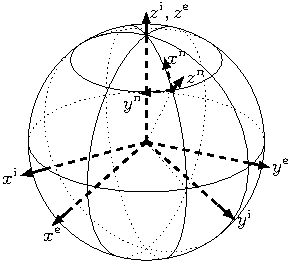
\includegraphics[scale = 1]{Coordinate systems.pdf}
    \caption{The $n$, $i$ and $e$ coordinate systems shown on the Earth.~\cite{Kok2017}}
\end{figure}

g is taken to be positive for the purposes of this paper.

The quaternion convention used is the Hamilton convention defined in~\cite{Sol2017}.

Axis angle is a parameterisation of \SO{3} which is defined as $[\m u\tran \ \phi]\tran$, where $\phi$ is the angle of rotation in radians and $\m u$ is a unit vector representing the axis of rotation.

\begin{figure}[h]
    \centering
    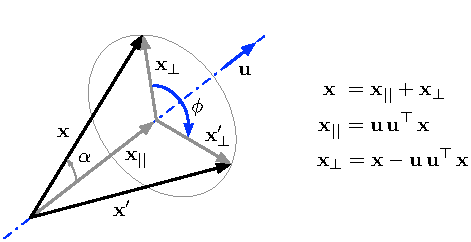
\includegraphics{rotation3d.pdf}
    \caption{The vector $\bf x$ rotated about $\bf u$ by $\phi$ gives vector $\bf x'$.\cite{Sol2017}}
\end{figure}

The skew symmetric matrix of a vector is defined as
\begin{align} \label{eq:crossProductMatrix}
    [\m{\omega}]_\times &\equiv \begin{bmatrix}
        0 & -\m{\omega}_z & \m{\omega}_y \\
        \m{\omega}_z & 0 & -\m{\omega}_x \\
        - \m{\omega}_y & \m{\omega}_x & 0
    \end{bmatrix}
\end{align}